\documentclass[12pt]{article}
 \usepackage[margin=1in]{geometry} 
\usepackage{amsmath,amsthm,amssymb,outlines}
\usepackage{graphicx,tikzsymbols,tcolorbox}
\usepackage{tikz,caption,subcaption}
\newcommand{\C}{\mathbb{C}}
\newcommand{\R}{\mathbb{R}}
\newcommand{\Z}{\mathbb{Z}}
\renewcommand\qedsymbol{$\blacksquare$}
\tcbuselibrary{most}

% Defining new environments

\newtcolorbox{newtitle}{
  enhanced,
  colframe=black,
  colback=white,
  boxsep=5pt,
  arc=8pt,
  borderline={0.5pt}{0pt}{black},
  borderline={1.8pt}{-5pt}{black},
  after skip=30pt
}

\newtcolorbox[auto counter, number within=section]{theorem}[2][title]{
  enhanced,
  title={Theorem \thetcbcounter \if\relax\detokenize{#2}\relax\else\ (#2)\fi},
  colframe=black,
  colback=white,
  colbacktitle=white,
  fonttitle=\bfseries,
  coltitle=black,
  attach boxed title to top left={yshift=-0.25mm-\tcboxedtitleheight/2,yshifttext=2mm-\tcboxedtitleheight/2, xshift=2mm},
  boxed title style={boxrule=0.5mm}
}

\newtcolorbox[]{definition}{
  enhanced,
  title={Definition \thetcbcounter},
  colframe=black,
  colback=white,
  colbacktitle=white,
  fonttitle=\bfseries,
  coltitle=black,
  attach boxed title to top left={yshift=-0.25mm-\tcboxedtitleheight/2,yshifttext=2mm-\tcboxedtitleheight/2, xshift=2mm},
  boxed title style={boxrule=0.5mm}
}

\newtcolorbox[auto counter, number within=section]{fact}{
  enhanced,
  title={Fact \thetcbcounter},
  colframe=black,
  colback=white,
  colbacktitle=white,
  fonttitle=\bfseries,
  coltitle=black,
  attach boxed title to top left={yshift=-0.25mm-\tcboxedtitleheight/2,yshifttext=2mm-\tcboxedtitleheight/2, xshift=2mm},
  boxed title style={boxrule=0.5mm}
}

\newtcolorbox[auto counter, number within=section]{notation}{
  enhanced,
  title={Notation},
  colframe=black,
  colback=white,
  colbacktitle=white,
  fonttitle=\bfseries,
  coltitle=black,
  attach boxed title to top left={yshift=-0.25mm-\tcboxedtitleheight/2,yshifttext=2mm-\tcboxedtitleheight/2, xshift=2mm},
  boxed title style={boxrule=0.5mm}
}

\newtcolorbox[auto counter]{statement}[1][]{
  enhanced,
  breakable,
  title={Problem \ifx\\#1\\\thetcbcounter\else#1\fi},
  colframe=black,
  colback=white,
  colbacktitle=white,
  fonttitle=\bfseries,
  coltitle=black,
  attach boxed title to top left={yshift=-0.25mm-\tcboxedtitleheight/2,yshifttext=2mm-\tcboxedtitleheight/2, xshift=2mm},
  boxed title style={boxrule=0.5mm}
}

\newtcolorbox{newproof}{
  enhanced,
  breakable,
  frame hidden,
  colback=white,
  title={Proof.},
  fonttitle=\bfseries,
  coltitle=black,
  colbacktitle=white,
  boxed title style={boxrule=0.5mm},
  attach boxed title to top left={yshift=-0.25mm-\tcboxedtitleheight/2,yshifttext=2mm-\tcboxedtitleheight/2, xshift=2mm},
  borderline west={1.5pt}{8pt}{black},
  after upper={\hfill $\blacksquare$}
}

\newtcolorbox[auto counter, number within=section]{uq}{
  enhanced,
  title=Question,
  colframe=red,
  colback=white,
  colbacktitle=white,
  fonttitle=\bfseries,
  coltitle=black,
  attach boxed title to top left={yshift=-0.25mm-\tcboxedtitleheight/2,yshifttext=2mm-\tcboxedtitleheight/2, xshift=2mm},
  boxed title style={boxrule=0.5mm}
}

\newtcolorbox[auto counter, number within=section]{aq}{
  enhanced,
  title=Question,
  colframe=black!50!black,
  colback=white,
  colbacktitle=white,
  fonttitle=\bfseries,
  coltitle=black,
  attach boxed title to top left={yshift=-0.25mm-\tcboxedtitleheight/2,yshifttext=2mm-\tcboxedtitleheight/2, xshift=2mm},
  boxed title style={boxrule=0.5mm}
}

\newtcolorbox{answer}{
  enhanced,
  frame hidden,
  colback=white,
  colframe=black!50!black,
  title={Answer},
  fonttitle=\bfseries,
  coltitle=black,
  colbacktitle=white,
  boxed title style={boxrule=0.5mm},
  attach boxed title to top left={yshift=-0.25mm-\tcboxedtitleheight/2,yshifttext=2mm-\tcboxedtitleheight/2, xshift=2mm},
  borderline west={1.5pt}{8pt}{black!50!black}
}

% Redefine section as well

% Renew commands later

\begin{document}

\begin{newtitle}
  \begin{center}
    \textbf{\Huge Topology Qual Cheat Sheet}
  \end{center}
  \textbf{Dahlen Elstran} \hfill \textbf{Spring 2025}
\end{newtitle}

\begin{center} \section*{Point Set Topology Definitions} \end{center}

\begin{definition}
  If $X$ is a topological space with topology $\mathcal{T}$, we say that a subset $U$ of $X$ 
  is an \textbf{open set} of $X$ if $U$ belongs to the collection $\mathcal{T}$.
\end{definition}

\begin{definition}
  A subset $A$ of a topological space $X$ is said to be \textbf{closed} if the set $x - A$ is open.
\end{definition}

\begin{definition}
  The \textbf{closure} of $A$ is defined as the intersection of all closed sets containing $A$.
\end{definition}

Casually, I like to think about it as the outer edge of the space, unioned with the space itself. For a closed space, like $[0,1]$, 
the closure is $\{0\} \cup \{1\}$, which is contained in the closed set. Note that all closed sets are equal to the closure of the
closed sets; this is because the smallest closed set containing a closed set $A$ is $A$ itself. 

\begin{notation}
  The closure of a set $A$ is denoted as $\bar{A}$.
\end{notation}

So for closed sets $A$, $\bar{A} = A$. Similarly, we have:

\begin{definition}
  The \textbf{interior} of $A$ is defined as the union of all open sets contained in $A$.
\end{definition}

\begin{notation}
  The interior of a set $A$ is denoted as $\text{Int} A$.
\end{notation}

For similar logic as before, for open sets $A$, $\text{Int} A = A$. 

\begin{definition}
  If $A$ is a subset of the topological space $X$ and if $x$ is a point of $X$. we say that $x$ is a
  \textbf{limit point/ cluster point/ point of accumulation} of $A$ if every neighborhood of $x$ intersects $A$ in some point other than 
  $x$ itself.
  \par You can also say $x$ is a limit point of $A$ if $x$ is in the closure of $A - \{ x \}$.
\end{definition}

A limit point is just a point on the boundary on a subspace $A$, although it doesn't necessarily have to be in $A$ itself. The 
limit points are kind of the boundary part of the closure. Hence the following theorem:

\begin{theorem}{}
  Let $A$ be a subset of the topological space $X$; let $A'$ be the set of all the limit points of $A$. Then 
  $$ \bar{A} = A \cup A'. $$
\end{theorem}

One can then consider the relationship between limit points and a set being closed. If the "boundary" of a set is 
made up of limit points, one can see that:

\begin{theorem}{}
  A subset of a topological space is closed if and only if it contains all its limit points.
\end{theorem}

\begin{definition}
  A collection $\mathcal{A}$ of subsets of a space $X$ is said to \textbf{cover} $X$, or to be a \textbf{covering} of $X$, if the union
  of the elements of $\mathcal{A}$ is equal to $X$. It is called an \textbf{open covering} of $X$ if its elements
  are open subsets of $X$.
\end{definition}

\begin{definition}
  A Space $X$ is said to be \textbf{compact} if every open covering $\mathcal{A}$ of $X$ contains a finite subcollection
  that also covers $X$. 
\end{definition}

\begin{definition}
  A topological space $X$ is called a \textbf{Hausdorff space} if for each pair $x_1,x_2$ of distinct points of $X$, 
  there exist neighborhoods $U_1$ and $U_2$ of $x_1$ and $x_2$ respectively that are disjoint.
\end{definition}

\begin{definition}
  Let $X$ be a topological space. A \textbf{separation} of $X$ is a pair $U, V$ of disjoint nonempty open subsets 
  of $X$ whose union is $X$. A space $X$ is said to be \textbf{connected} if there does not exist a separation 
  of $X$.
\end{definition}

This is really as simple as it sounds. Examples:

INSERT IPAD DRAWING HERE

\begin{definition}
  A space is called \textbf{path connected} if every pair of points in $X$ can be joined by a path in $X$
\end{definition}

\begin{uq}
  So how is there a difference between being path connected and connected? Shouldn't being connected, so that
  the space has no disjoint parts, be enough to say that a path can be drawn from point to point?
\end{uq}

\begin{answer}
  The biggest example is the \textbf{Topologists sine curve}:
  $$ y(x) = 
    \begin{cases}
      \sin\left( \frac{1}{x} \right) & \text{if } 0 < x < 1, \\
      0 & \text{if } x = 0,
    \end{cases} $$ 
  This is a curve that is connected, but \textbf{not} path connected.
  Proof of connectedness:

  \par I'm not exactly sure why this works, but my thoughts are just because you technically can't find any separation 
  between the two parts, because the limit of $\sin{\frac{1}{x}}$ as $x \to 0$ from the right is 0; however, because there 
  is not actually any connected, you cannot draw a path. At least that's what I'm getting from this right now. 
\end{answer}

\newpage

\section*{Algebraic Topology Definitions}

\begin{definition}
  A map is \textbf{nullhomotopic} if it is homotopic to a constant map.
\end{definition}

\begin{definition}
  A space is \textbf{contractible} if it is homotopically equivalent to a point. 
\end{definition}

So it's contractible if it can homotopically be squeezed into a point. 

\begin{theorem}{}
  A space is contractible if and only if it's identity map is nullhomotopic.
\end{theorem}
\begin{newproof}
  \begin{itemize}
    \item[($\implies$)] Assume a space $X$ is contractible, so that $X$ is homotopically equivalent to a point $x_0$. 
      Then there exists maps $f: X \to x_0$, $g:x_0 \to X$ such that $g \circ f \cong \text{id}_X$. But $g \circ f: X 
      \to X, x \mapsto x_0$, making it a constant map.
    \item[($\impliedby$)] If the identity map is nullhomotopic, it is homotopic to a constant map. This is 
      equivalent to saying there exists some $F(x,t)$ such that $F(x,0) = \text{id}_X$ and $F(x,1) = x_0 \forall x \in X$.
      This homotopy describes the space $X$ contracting to the point $x_0$ continuously.
  \end{itemize}
\end{newproof}

The backwards direction of this proof seems hand-wavey, so I may need to go back and look at this. 

\begin{definition}
  A space is called \textbf{simply connected} if it is path connected and has trivial fundamental group
\end{definition}

So a space is simply connected if there's nothing on the inside of it that causes loops to get "caught" on 
things. The first example that comes to my mind is how $S^2$ is simply connected, because it is path connected clearly, 
and any loop on $S^2$ can be contracted to a point (trivial fundamental group). On the other hand, the torus is path
connected, but a loop could be caught around the donut hole in the middle, unable to contract, resulting in a nontrivial 
fundamental group ($\Z \times \Z$, specifically).

\begin{definition}
  For a space $X$ to be \textbf{locally path-connected}, for each point $x \in X$ and each neighborhood $U$ of $x$, there must 
  be an open neighborhood $V \subset U$ of $x$ that is path-connected.
\end{definition}

A good example of this would be two disjoint discs. Clearly, the space itself isn't path connected, but the two components are 
path-connected themselves, so the space is locally path-connected.

\begin{aq}
  So why is $p$ from $\tilde{X}$ to $X$? To me, it seems more natural to assign $x \in X$ to somewhere in the cover. 
\end{aq}
\begin{answer}
  A cover could have more than one sheet, so that each $x \in X$ maps to multiple $\tilde{x} \in \tilde{X}$. Thus $p$ would 
  not be a function if it went from $X$ to $\tilde{X}$ for multi-sheeted covering spaces. 
\end{answer}
\begin{theorem}{Homotopy Lifting Property}
  Given a covering space $p: \tilde{Y} \to Y$, a homotopy $f_t: X \to Y$, and a map $\tilde{f_0}: X \to \tilde{Y}$ lifting $f_0$, 
  then there exists a unique homotopy $\tilde{f}_t:X \to \tilde{Y}$ of $\tilde{f}_0$ that lifts $f_t$.
\end{theorem}

\begin{theorem}{Lifting Criterion}
  Suppose given a covering space $p:(\tilde{Y},\tilde{y}_0) \to (Y, y_0)$ and a map $f:(X,x_0) \to (Y, y_0)$ with 
  $X$ path-connected and locally path-connected. Then a lift $\tilde{f}: (X,x_0) \to (\tilde{Y}, \tilde{y}_0)$ 
  of $f$ exists if and only if $f_*(\pi_1(X,x_0)) \subset p_*(\pi_1(\tilde{Y},\tilde{y}_0))$.
\end{theorem}
\begin{aq}
  So what is $p_*(\pi_1(\tilde{Y},\tilde{y}_0))$?
\end{aq}
\begin{answer}
  First note that $(\tilde{Y}, \tilde{y}_0)$ is the covering space of $Y$ and it's matching basepoint $y_0$ in the cover. 
  Obviously, $\pi_1(\tilde{Y},\tilde{y}_0)$ is the fundamental group of this covering space, and $p: (\tilde{Y}, \tilde{y}_0) 
  \to (Y,y_0)$ is the map that describes how the covering space covers $Y$, so $p_*$ is the induced homomorphism of the 
  fundamental groups. So $p_*(\pi_1(\tilde{Y},\tilde{y}_0))$ are the values in the codomain that are actually mapped to, or 
  $\text{img}(p_*)$. Note that $\text{img}(p_*) \subset \pi_1(Y,y_0)$, just like $f_*(\pi_1(X,x_0)) = \text{img}(f_*) \subset 
  \pi_1(Y,y_0)$, which makes sense.
\end{answer}

Given this, we can look at this diagram to see the relationship between $X$,$Y$ and $\tilde{Y}$: 

\par \begin{center} 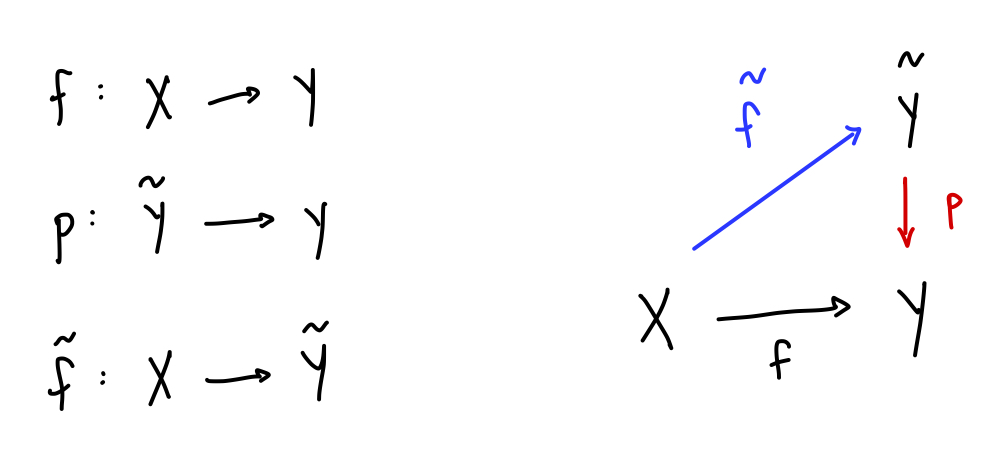
\includegraphics[scale=.2]{pics/liftcomposition} \end{center} 

And there is a similar setup for their respective fundamental groups:

\par \begin{center} 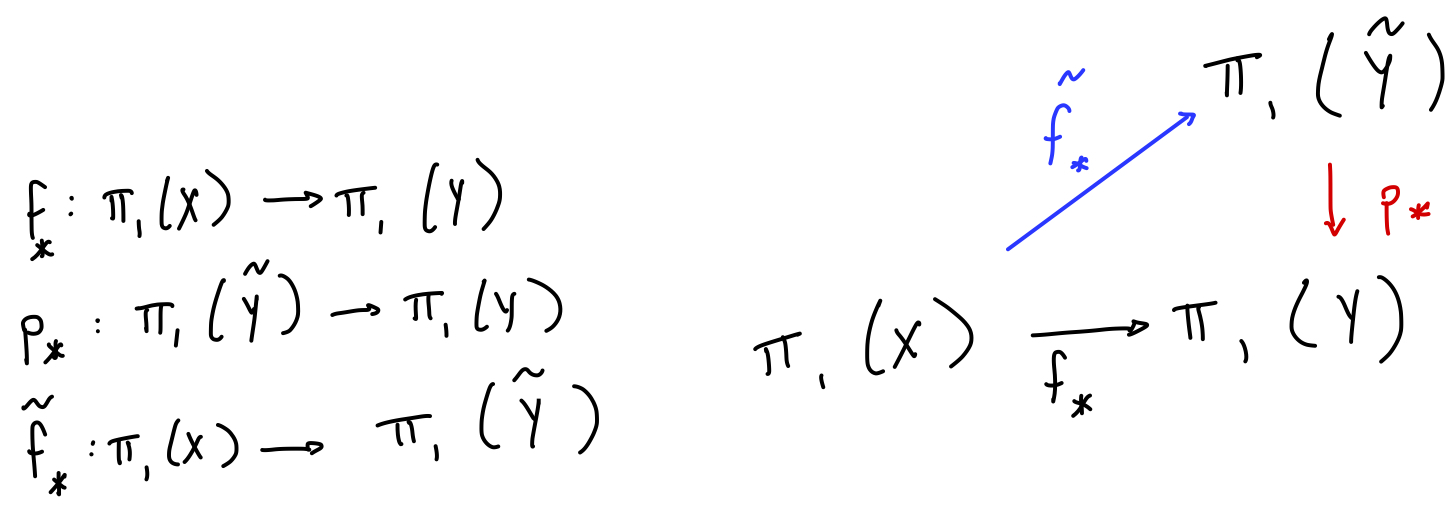
\includegraphics[scale=.2]{pics/inducedliftcomposition} \end{center} 

\begin{fact}
  By the diagrams above, we can see $f = p \circ \tilde{f}$ and $f_* = p_* \circ \tilde{f}_*$.
\end{fact}

\begin{uq}
  So what determines whether or not we can assume that $f$ is this composition? Is there some property to satisfy?
\end{uq}

\newpage

\section*{Qualifying Exams}

\subsection*{Spring 2025}

\begin{statement}
  Prove that any map $\R P^2 \to S^1 \times S^1$ is nullhomotopic. Prove that there exists a map $S^1 \times S^1 \to \R P^2$ which 
  is not nullhomotopic.
\end{statement}
\begin{newproof}
  The universal cover of $S^1 \times S^1$ is $\R \times \R$. So if $f:\R P^2 \to S^1 \times S^1$, the lifted map $\tilde{f}: \R P^2 \to \R 
  \times \R$ is nullhomotopic, since $\R \times \R$ is contractible. If the lifted map $\tilde{f}$ is nullhomotopic,
  then the map $f$ must be. So all that is left to show is that we can lift the map, so we must meet the lifting 
  criterion.
  \par The fundamental group of $S^1 \times S^1$ is $\Z \times \Z$, and the fundamental group of $\R P^2$ is $\Z / 2 \Z$, 
  as can be seen by the following diagrams:
  \par INSERT IPAD DRAWINGS HERE
  \par Then $f$ induces a homomorphism $f_*: \pi_1(\R P^2) \to \pi_1(S^1 \times S^1)$, which is clearly trivial. 
  Then we know $f_*(\pi_1(X,x_0)) \subset p_*(\pi_1(\tilde{Y},\tilde{y}_0))$, because $f_*(\pi_1(X,x_0))=f_*(\Z / 2\Z)=0$, and
  $p_*(\pi_1(\tilde{Y},\tilde{y}_0))=p_*(\pi_1(\R \times \R))=p_*(0)=0$. We must also show that $\R P^2$ is path-connected 
  and locally path-connected, but this is obvious as it is a quotient space of $S^2$, and $S^2$ has those properties.
  Thus the lifting criterion is met, 
  and $f$ must be nullhomotopic.
\end{newproof}
\begin{aq}
  Why do we need the fundamental groups? Why can't we just say that the lifted map is nullhomotopic, so the 
  normal map must be to?
\end{aq}
\begin{answer}
  We have to prove the lift exists, and so we must satisfy the lifting criterion.
\end{answer}
\begin{aq}
  Why does any map $f: \Z / 2\Z \to \Z \times \Z$ have to be trivial?
\end{aq}
\begin{answer}
  We know that $\Z / 2 \Z$, or $\Z_2$ has two elements, $\{0,1\}$. We know because $f$ is a homomorphism,
  $f(0)=0$. Then $f(1)$ must satisfy $f(1 + 1) = f(1) + f(1)$, but $1+1=0$ in $\Z_2$, so we have 
  $f(1) + f(1) = 0$, and because $\Z \times \Z$ is \textbf{torsion-free} (there are no non-identity elements that have 
  finite order (so like there are no non-identity elements that can every generate the identity by themselves)),
  the only values $f(1)$ can take on to follow this restriction is 0. Thus every element in $\Z_2$ maps to 0, and 
  $f$ must be trivial.
\end{answer}
\begin{aq}
  So why does the lift being nullhomotopic imply the original is nullhomotopic?
\end{aq}
\begin{answer}
  So we know $tilde{f} \cong c_1$, where $c_1$ is a constant map. But $f = p \circ \tilde{f} \cong p \circ c_1$, so for 
  $f$ to be nullhomotopic, $p$ must be nullhomotopic too. But because $p:\R \times \R \to S^1 \times S^1$, and 
  $\R \times \R$ is contractible, $p$ is nullhomotopic as well, so that $p \cong c_2$ for some constant map $c_2$. 
  Thus $f \cong c_2 \circ c_1$, so that $f$ is nullhomotopic.
\end{answer}

\newpage

\section*{Blank Problem Bank}

\subsection*{Homework 1}

\begin{statement}[0.2]
    Construct an explicit deformation retraction of $\mathbb{R}^n - \{0\}$ onto $S^{n-1}$.
\end{statement}

\begin{statement}[0.3]
    \begin{itemize}
        \item[(a)] Show that the composition of homotopy equivalences $X \to Y$ and $Y \to Z$ is a homotopy equivalence $X \to Z$. Deduce that homotopy equivalence is an equivalence relation.

        \item[(b)] Show that the relation of homotopy among maps $X \to Y$ is an equivalence relation.

        \item[(c)] Show that a map homotopic to a homotopy equivalence is a homotopy equivalence.
    \end{itemize}
\end{statement}

\begin{statement}[0.6]
  \begin{itemize}
    \item[(a)] Let $X$ be the subspace of $\R^2$ consisting of the horizontal segment $[0,1] \times \{0\}$ 
      together with all the vertical segments $\{r\} \times [0,1-r]$ for $r$ a rational number in 
      $[0,1]$. Show that $X$ deformation retracts to any point in the segment $[0,1] \times \{ 0\}$, but
      not to any other point. [See the preceding problem]
    \item[(b)] Let $Y$ be the subspace of $\R^2$ that is the union of an infinite number of copies of $X$ 
      arranged as in the figure below. Show that $Y$ is contractible but does not deformation retract 
      onto any point. 
    \item[(c)] Let $Z$ be the zigzag subspace of $Y$ homeomorphic to $/R$ indicated by the heavier line. 
      Show there is a deformation retraction in the weak sense (see Exercise 4) of $Y$ onto $Z$, but no true 
      deformation retraction.
  \end{itemize}
\end{statement}

\begin{statement}[0.10]
    Show that a space $X$ is contractible if and only if every map $f:X \to Y$, for arbitrary $Y$, is nullhomotopic. Similarly, show $X$ is contractible if and only if every map $f: Y \to X$ is nullhomotopic.
\end{statement}

\begin{statement}[0.11]
    Show that $f: X \to Y$ is a homotopy equivalence if there exist maps $g,h:Y \to X$ such that $fg \cong \text{id}$ and $hf \cong \text{id}$. More generally, show that $f$ is a homotopy equivalence if $fg$ and $hf$ are homotopy equivalences. 
\end{statement}

\begin{statement}[0.16]
  Show that $S^{\infty}$ is contractible.
\end{statement}

\begin{statement}[0.17]
    Construct a 2-dimensional cellcomplex that contains both an annulus $S^1 \times I$ and a Mobius band as 
    deformation retractions.
\end{statement}

\begin{statement}[0.20]
    Show that the subspace $X \subset \mathbb{R}^3$ formed by a Klein bottle intersecting itself in a circle is homotopy equivalent to $S^1 \vee S^1 \vee S^1$.
\end{statement}

\newpage

\section*{Notes}

\subsection*{Mayer-Vietorus}

You take a space $X$, find an $A$ and a $B$ such that $A \cup B = X$ and $A \cap B$ is open.

Then you can set up a long exact sequence. 

FINISH LATER

\subsection*{Van Kampen}

Like MV for fundamental groups, you look for an $A$ and $B$ with an open intersection. Look for 
any identifications in the intersection.

FINISH LATER

\subsection*{Classification of Surfaces}

Good blog post

Euler Characteristic: $\xi(X) = \text{# of 0-cells} - \text{# of 1-cells} + \text{# of 2-cells}$

Genus for nonorientable: 

\end{document}
